%%%%%%%%%%%%%%%%%%%%%%%%%%%%%%%%%%%%%%%%%%%%%%%%%%%%%%%%%%%%%%%%%%%%%%
%     File: ExtendedAbstract_resul.tex                               %
%     Tex Master: ExtendedAbstract.tex                               %
%                                                                    %
%     Author: Andre Calado Marta                                     %
%     Last modified : 27 Dez 2011                                    %
%%%%%%%%%%%%%%%%%%%%%%%%%%%%%%%%%%%%%%%%%%%%%%%%%%%%%%%%%%%%%%%%%%%%%%
% Results
% Results should be clear and concise.
% Discussion
% This should explore the significance of the results of the work, not
% repeat them. A combined Results and Discussion section is often
% appropriate. Avoid extensive citations and discussion of published
% literature.
%%%%%%%%%%%%%%%%%%%%%%%%%%%%%%%%%%%%%%%%%%%%%%%%%%%%%%%%%%%%%%%%%%%%%%

\section{Results}
\label{sec:resul}
We are now able to train the models on the aforementioned data using the implementation methods described before.

We begin by showing in \autoref{fig:DupLocVol} the local volatility surface resulting from the Dupire's local volatility model, which we obtained by interpolating the implied volatility data and applying Dupire's formula. This surface can then be used in a Monte Carlo pricer, as we explained before.


\begin{figure}[H]
    \centering
      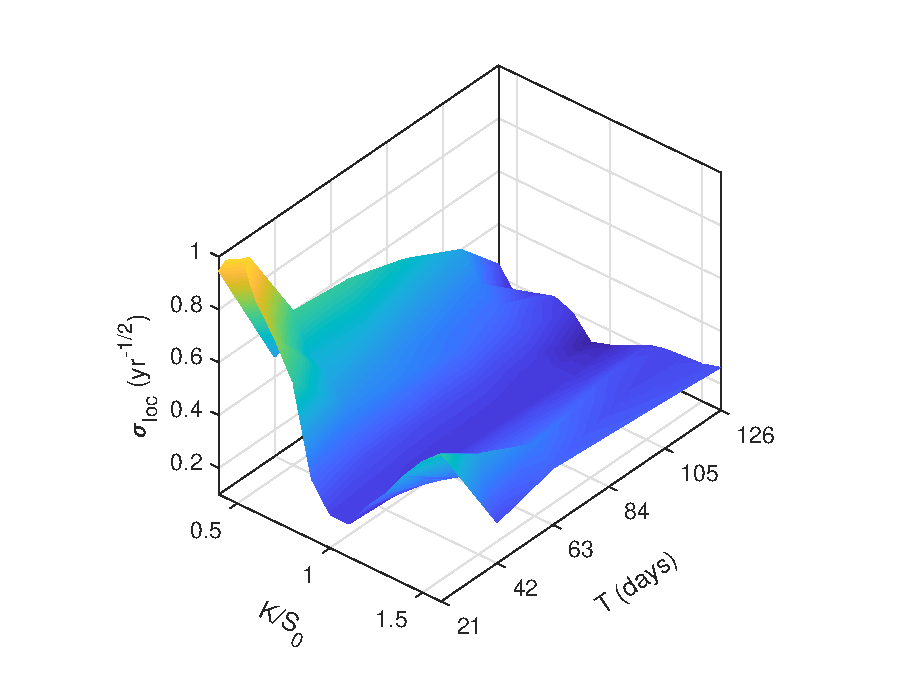
\includegraphics[width=.8\columnwidth,trim={1.7cm 0.45cm 2.cm 0.85cm},clip]{LocalV.eps}
      \caption{Local volatility surface obtained with Dupire's formula}\label{fig:DupLocVol}
    \end{figure}
    
    
Regarding now the stochastic volatility models, we calibrated them with the cost function described before using the CMA-ES optimization algorithm. The calibrated parameters for these models are represented in Tables \ref{tab:SSR}-\ref{tab:DSR}, with the resulting costs in \autoref{tab:CostsCompare}.
 
We should note that the Static SABR model was trained on data for each maturity independently, whereas the Heston and Dynamic SABR models were trained on all maturities together dependently, as an ensemble. In other words, the Static SABR model was trained 4 times (once for each maturity) on a data set of 7 implied volatilities (with different strikes), whereas Heston and Dynamic SABR were trained on a data set of 28 (7$\times$4) implied volatilities, disregarding maturity. For this reason, in \autoref{tab:CostsCompare}, for the Static SABR model we show the sum of the costs of calibration on each maturity, $\Sigma_{\mathrm{Costs}}$.

To have a benchmark for how well each model performs, we also trained a constant volatility model twice, with the calibration done independently for each maturity, as for Static SABR, and dependently, like Heston. Because the calibrated constant volatilities are not relevant for our results, they are not shown here, though we represent their costs in \autoref{tab:CostsCompare}.


\begin{table}[H]
    \centering
        \renewcommand{\arraystretch}{0.8}
\begin{tabular}{@{}lcccr@{}}
\toprule
 $T$(days) & $\alpha$($\SI{}{\year\tothe{-0.5}}$) & $\beta$ & $\rho$ & $\nu$($\SI{}{\year\tothe{-0.5}}$)  \\ \midrule
21 & 0.24 & 0.38 & -0.38 & 2.10 \\
42 & 0.24 & 0.74 & -0.37 & 1.45\\
63 & 0.24 & 0.78 & -0.31 & 1.14\\
126& 0.23 & 0.88 & -0.24 & 0.82\\
\bottomrule
\end{tabular}
  \caption{Fitted parameters for each maturity (fitted independently) under Static SABR model.}
  \label{tab:SSR}
\end{table}

\begin{table}[H]
    \centering
        \renewcommand{\arraystretch}{0.8}
\begin{tabular}{@{}lcccr@{}}
\toprule
$\kappa$($\SI{}{\year\tothe{-1}}$) & $\overline{\nu}$($\SI{}{\year\tothe{-1}}$) & $\nu_0$($\SI{}{\year\tothe{-1}}$) & $\rho$ & $\eta$($\SI{}{\year\tothe{-1}}$)  \\ \midrule
53.44 & 0.07 & 0.10 & -0.41 & 6.26  \\
\bottomrule
\end{tabular}
  \caption{Fitted parameters for all maturities (fitted simultaneously) under the Heston model.}
  \label{tab:HR}
\end{table}

\begin{table}[H]
    \centering
        \renewcommand{\arraystretch}{0.8}
\begin{tabular}{@{}lccccr@{}}
\toprule
$\alpha$($\SI{}{\year\tothe{-0.5}}$) & $\beta$ & $\rho_0$ & $a$($\SI{}{\year\tothe{-1}}$) & $\nu_0$($\SI{}{\year\tothe{-0.5}}$) & $b$($\SI{}{\year\tothe{-1}}$)  \\ \midrule
0.25 & 0.63 & -0.42 & 0 & 1.87 & 41.69 \\
\bottomrule
\end{tabular}
  \caption{Fitted parameters for all maturities (fitted simultaneously) under the Dynamic SABR model.}
  \label{tab:DSR}
\end{table}


\begin{table}[H]
    \centering
        \renewcommand{\arraystretch}{0.8}
\begin{tabular}{@{}lcr@{}}
\toprule
 Model & Cost & $\Sigma_{\mathrm{Costs}}$ \\ \midrule
Constant Vol. (indep.) & - & 0.1150 \\
Constant Vol. (dep.) & 0.1248 & - \\
Dupire & - & - \\
Static SABR & - & 0.0008 \\
Heston & 0.0025 & - \\
Dynamic SABR & 0.0108\\
\bottomrule
\end{tabular}
  \caption{Comparison between the costs from the calibrated stochastic volatility models.}
  \label{tab:CostsCompare}
\end{table} 
 
We now analyze the calibration results presented before for the stochastic volatility models.

Starting with Static SABR, we first note that the cost after calibration is extremely low, showing an improvement of $99.3\%$ over the cost of the constant volatility model (with independent fits). This seems to suggest that the model fits the data almost perfectly, though this conclusion should be taken carefully: we have an extremely small amount of data points (7 for each maturity) for the comparatively large number of parameters used (4 parameters in total). This will cause our model to overfit the data, explaining our very low costs. To further corroborate this hypothesis, we note that the parameter $\beta$, which is expected to remain constant, varies wildly between maturities.
Finally, we note that, as expected, the parameter $\rho$ is always negative and that both $\rho$ and $\nu$ seem to tend to zero with time, validating the hypothesis from Fernandez \textit{et al.}
 

Regarding now the Heston model, we first emphasize the low cost value after calibration, with an improvement of $98.0\%$ over the constant volatility model (with dependent fits), which suggests that this model fits the data very well, without the overfitting problem from Static SABR.
The parameter $\kappa$ is very large, which means that the variance process ($\nu(t)=(\sigma(t))^2$) tends to its mean value, $\overline{\nu}$, very fast and that $\nu_0$ has almost no influence. Furthermore $\rho$ is negative, as expected, and $\eta$ is very large meaning that the variance process will be quite erratic.
 
Considering the Dynamic SABR model, the improvement of the cost value over the constant volatility model (with dependent fits) is now (only) $91.3\%$.
The parameter $a$ being $0$ implies that the function $\rho(t)$ is stuck at $\rho_0$, and the parameter $b$ being very large means that $\nu(t)$ goes to $0$ extremely fast. These results are very inconsistent with what is observed in the Static SABR model, where the $\rho$ and $\nu$ tend (slowly) to zero with time. This seems to suggest that the functions chosen to model these two parameters were not appropriate.


Finally, comparing all the stochastic volatility models, we can say that even though the Static SABR model presented the lowest cost, because of the mentioned overfitting, the Heston model might be the one that performs best among the three.
 
 
 
 
 
Having trained the models we are now able to simulate the results to produce forecasts and compare the models' simulations with one another.
The simulations were performed for all four maturities mentioned before, but, due to redundancy, we only show the plots for the first maturity of 1 month.

Regarding Dupire's local volatility model, having obtained the local volatility surface we are able to simulate the stock price paths with the discretization method described before. From these, we can extract the implied volatilities for many different strikes (converting them from option prices). These simulations are performed $100$ times for each strike and then averaged to produce the \emph{simulated function}, as shown in Figure \ref{fig:Dup1}. The simulations don't always produce the exact same results and some variation might occur. To represent this variation we also show the 95\% \emph{confidence bands} of the simulations in the plot (i.e. 95\% of all observations are contained within these bands). In the same plot we also represent the implied volatility data for the first maturity.

Considering the stochastic volatility models, we show the same information as for Dupire's model but we also include the calibrated closed form solutions, which we call \emph{theoretical functions}.


To run the Monte Carlo pricers we used an initial stock price of $S_0=1\text{\euro}$, a risk-free interest rate $r=0$, a time step size $\Delta t=0.5$\ days and simulated a total of 100\ 000 paths.

\newpage
    
\begin{figure}[H]
  \begin{subfigmatrix}{1}
    \subfigure[Dupire's model]{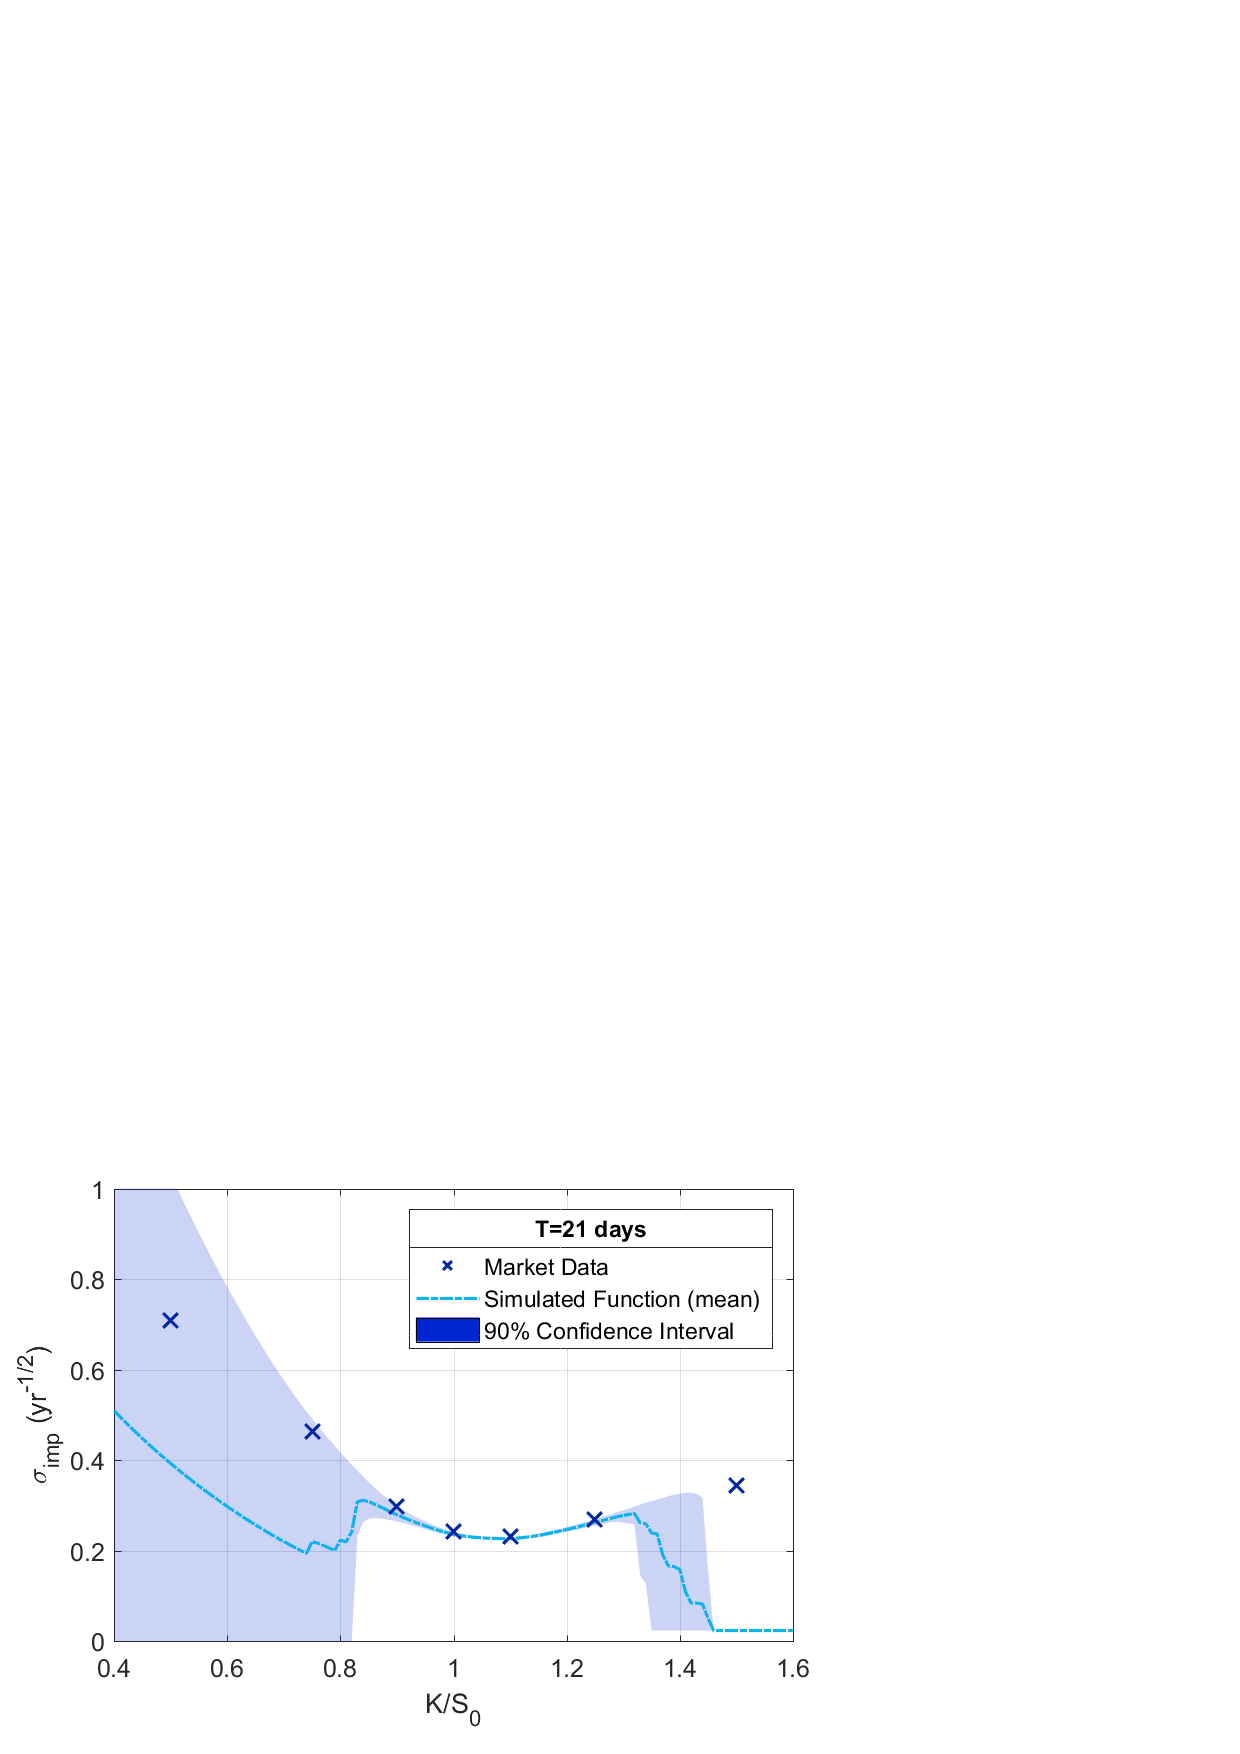
\includegraphics[width=.95\columnwidth,trim={0.25cm 0.45cm 1.1cm 1.4cm},clip]{Dup1.png}\label{fig:Dup1}}
    \subfigure[Static SABR]{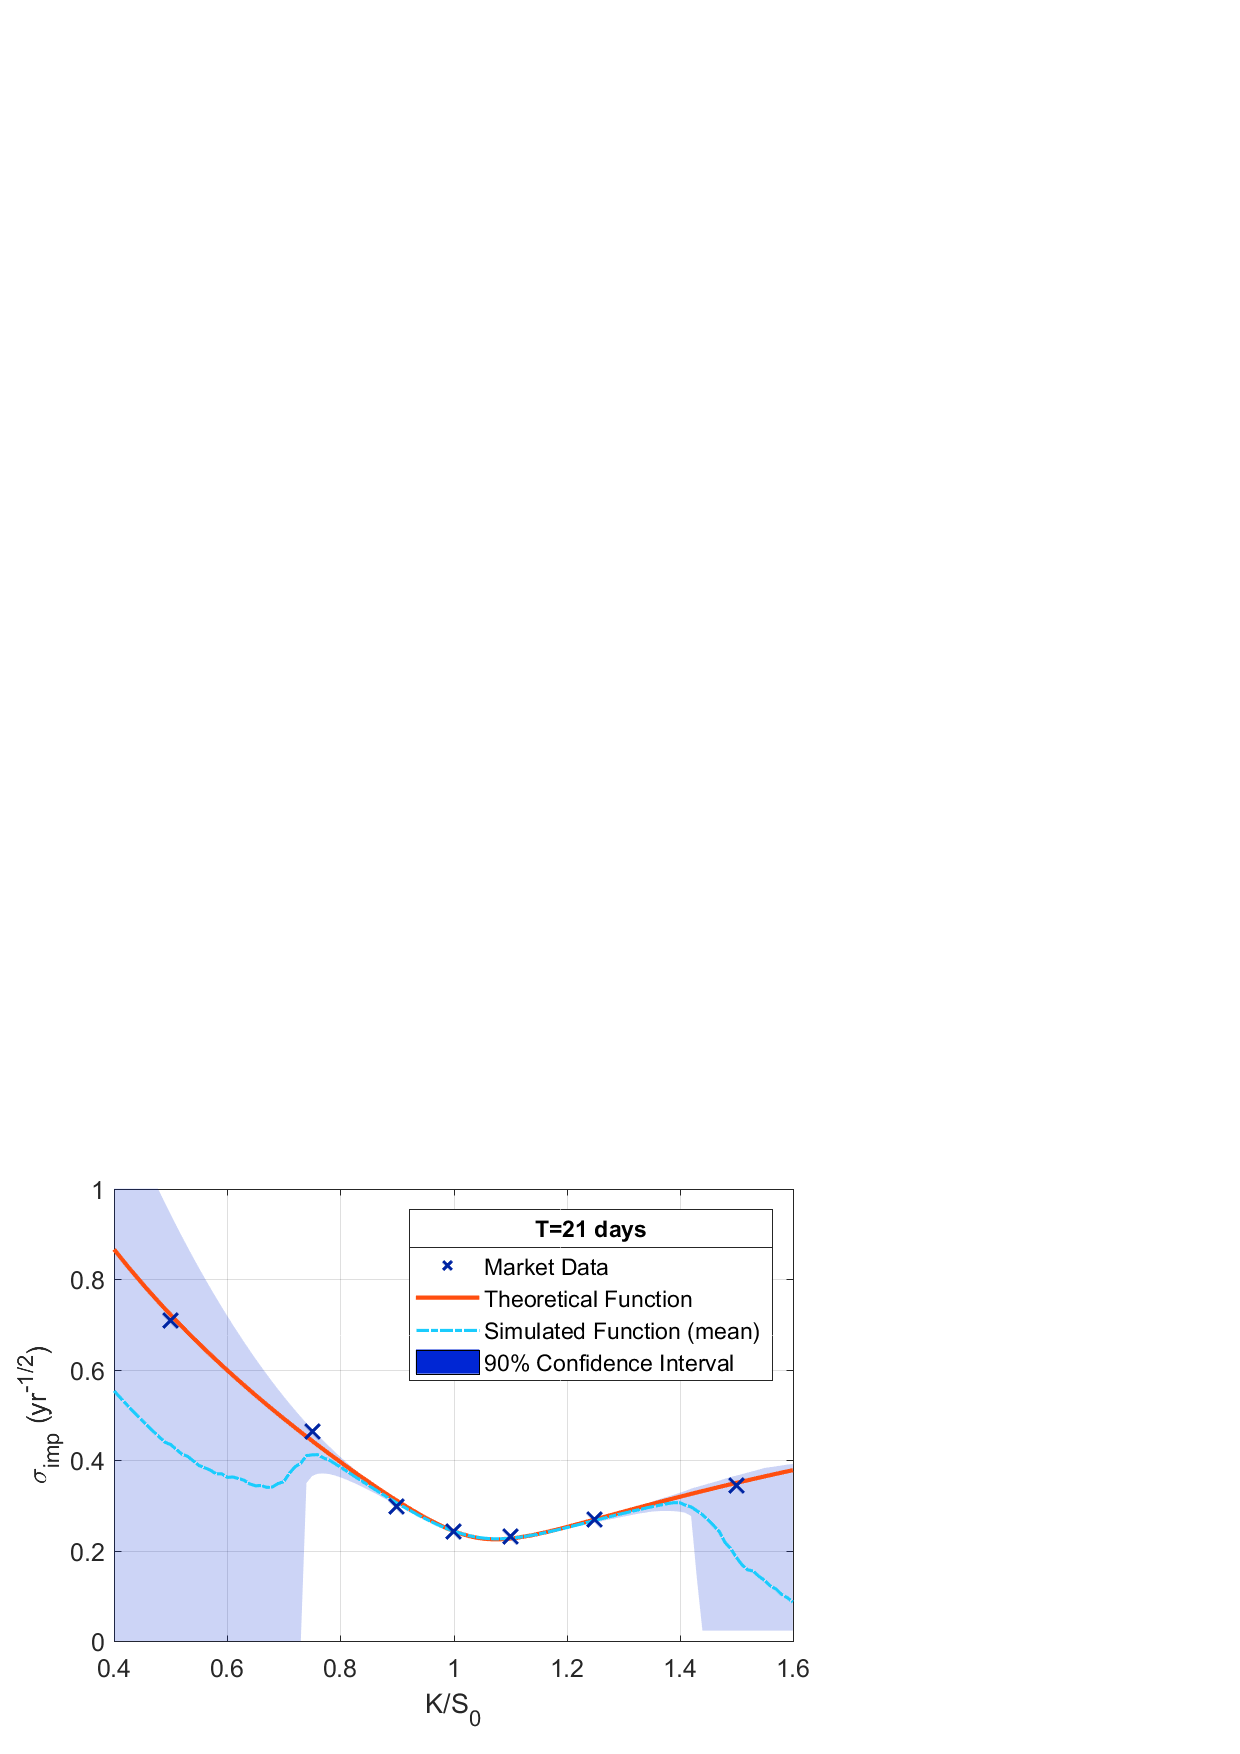
\includegraphics[width=.95\columnwidth,trim={0.25cm 0.45cm 1.1cm 1.4cm},clip]{SSABR1.png}}
    \subfigure[Heston model]{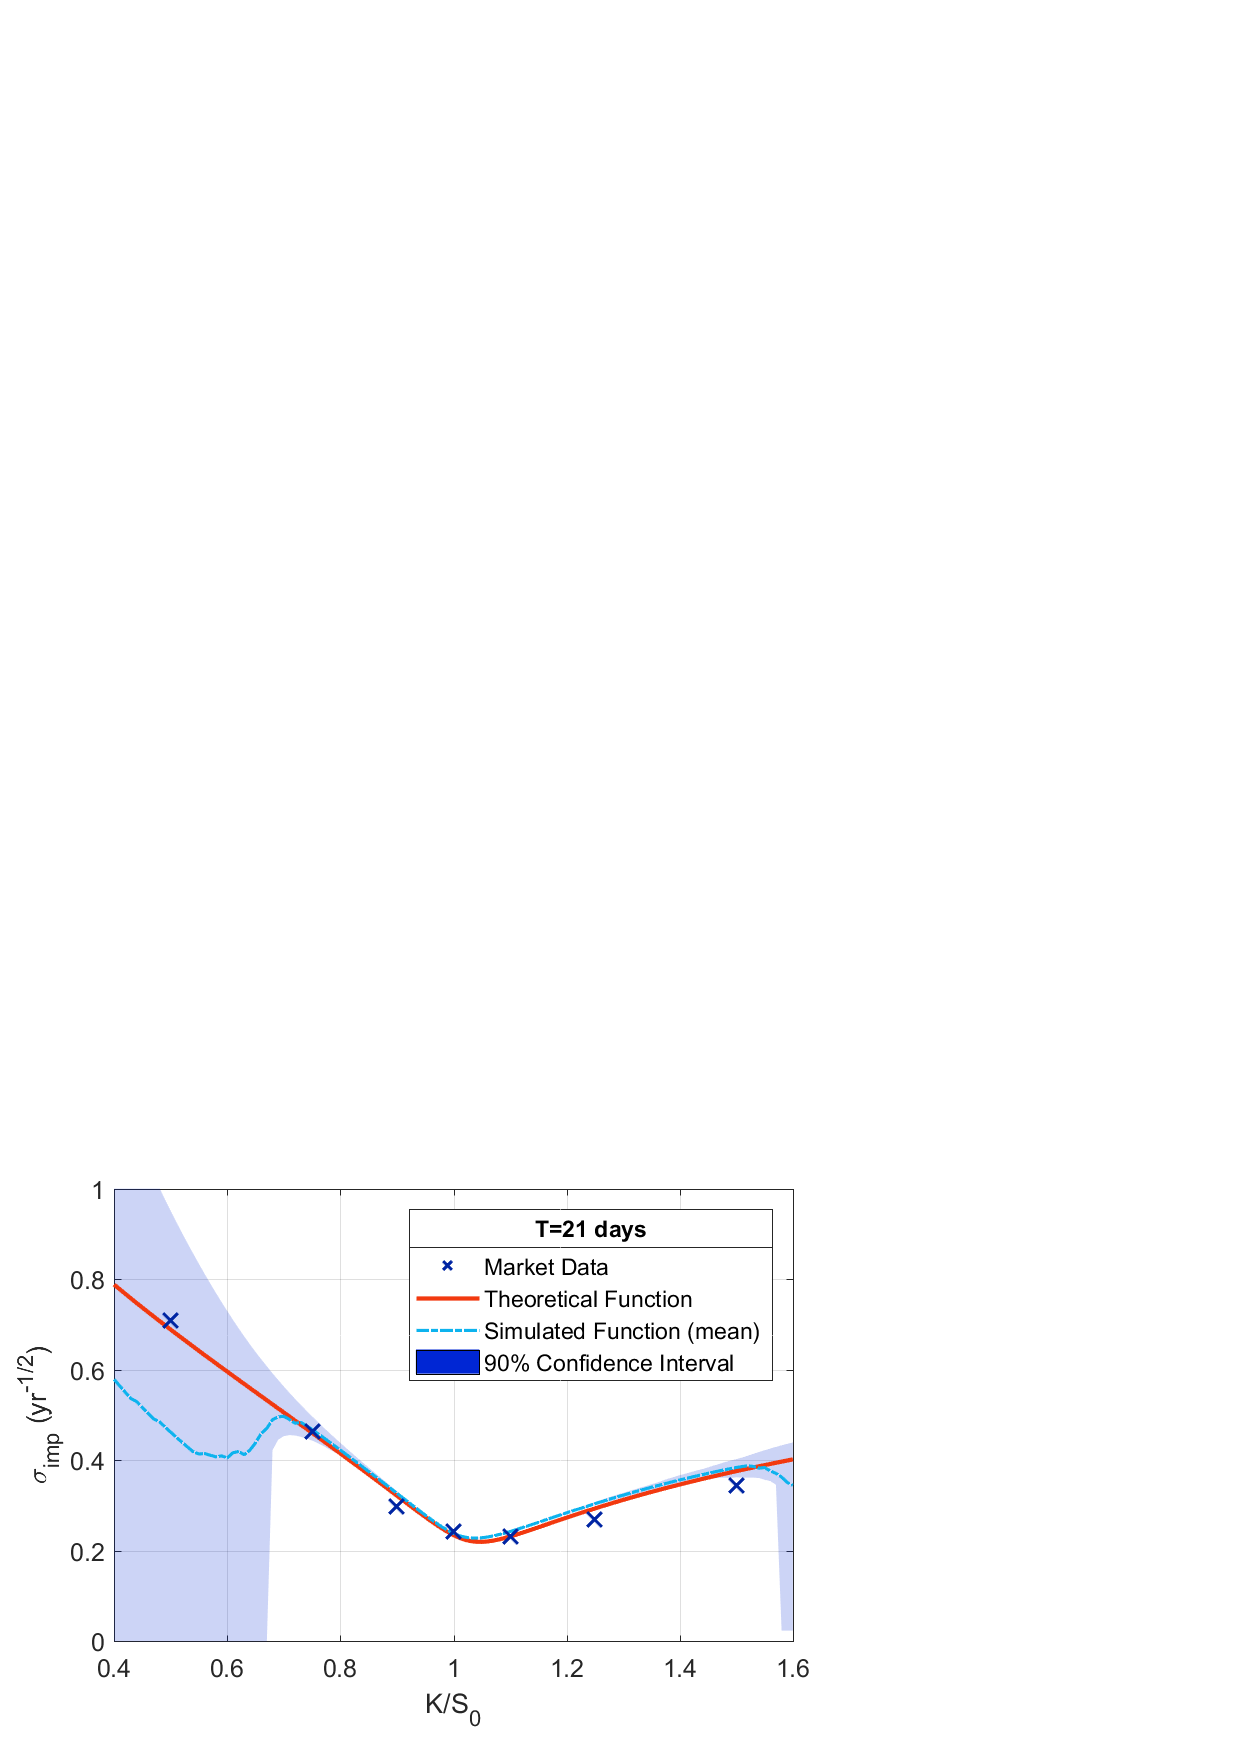
\includegraphics[width=.95\columnwidth,trim={0.25cm 0.45cm 1.1cm 1.4cm},clip]{H1.png}}
    \subfigure[Dynamic SABR]{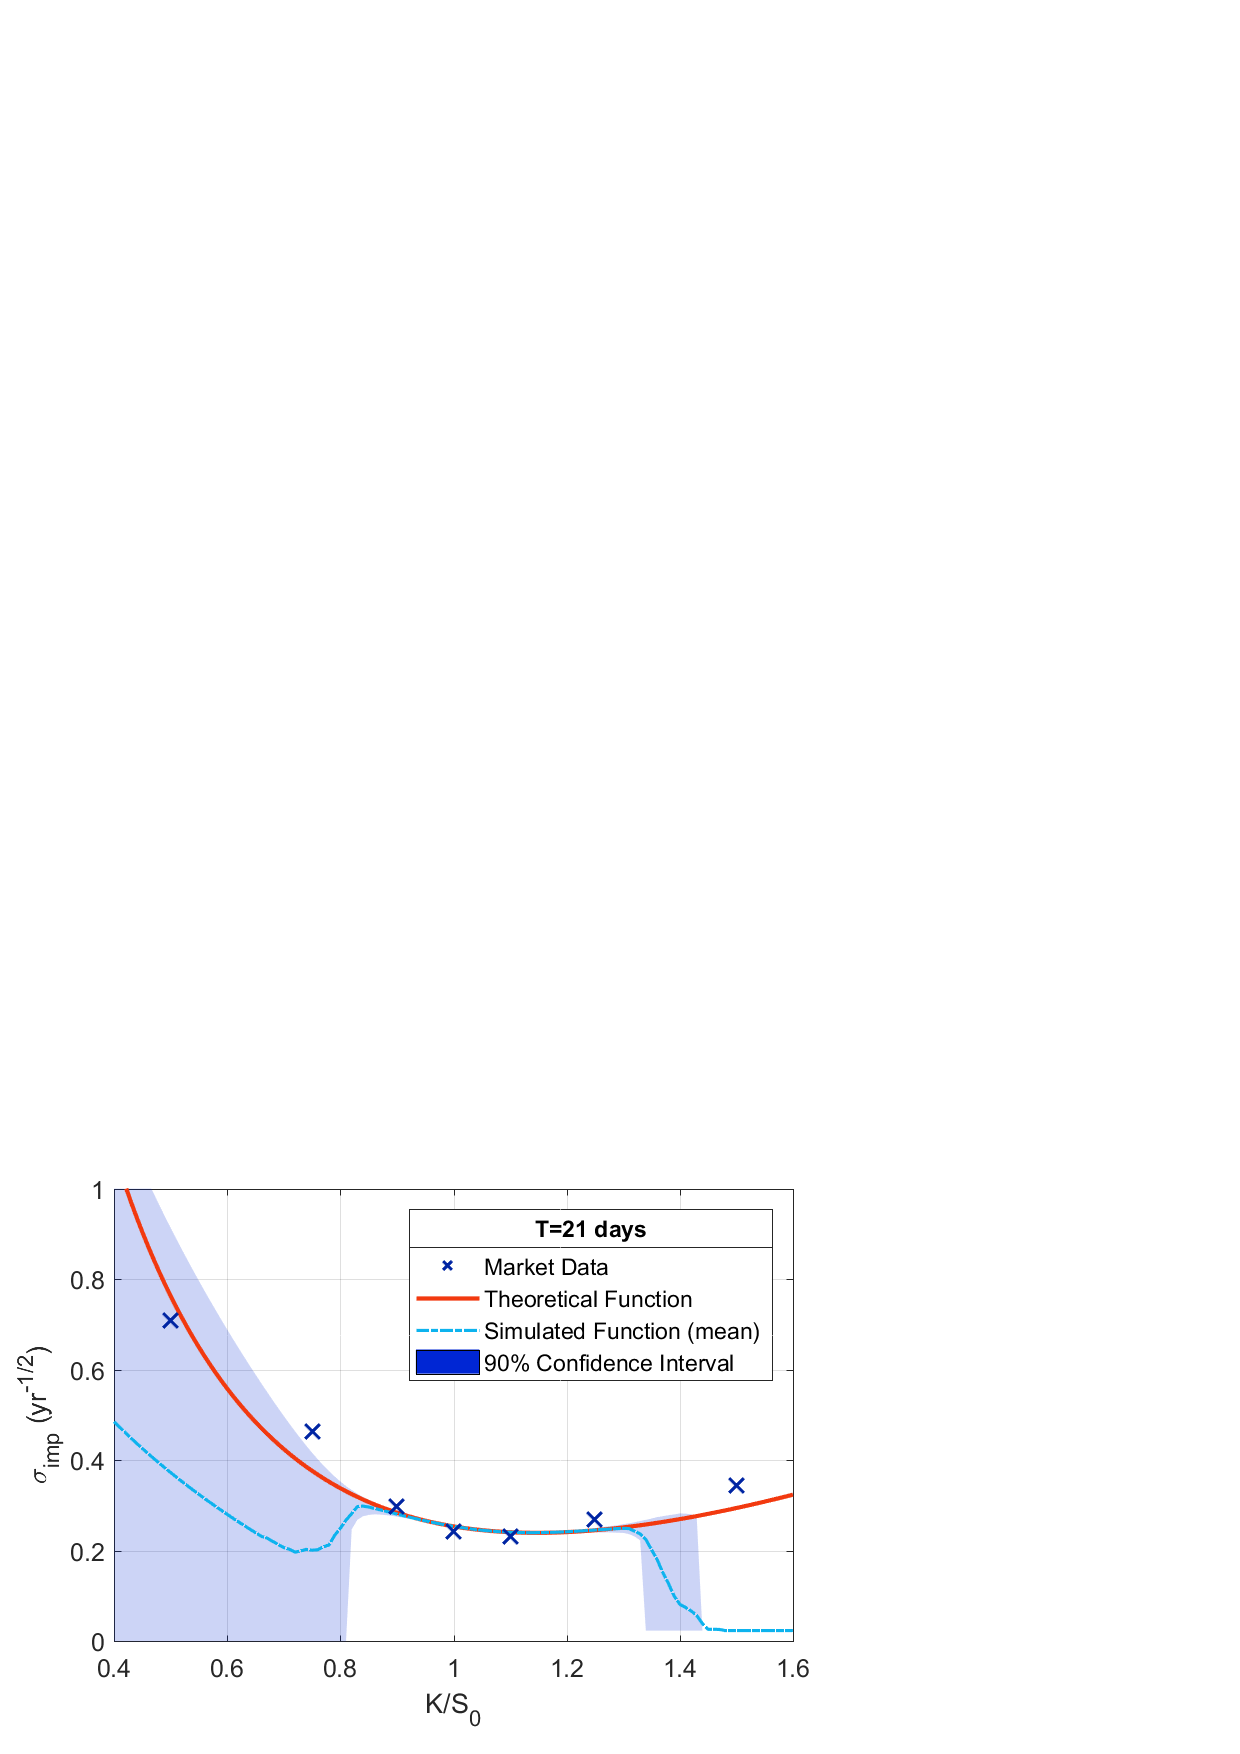
\includegraphics[width=.95\columnwidth,trim={0.25cm 0.45cm 1.1cm 1.4cm},clip]{DS1.png}}
  \end{subfigmatrix}
  \caption{Simulations and closed-form solutions under each model}
\end{figure}
    
We now analyze the results shown in the previous plots.

We begin by noting that in the regions with strikes around $S_0$ all simulations follow the closed form solutions very closely, with almost no variation, which seems to suggest that the implementation was done correctly for all models. Furthermore, all models match the implied volatility data quite well in this region.

Regarding the simulated functions, we can see that they decrease significantly for large strikes, presenting also a large variation (i.e. wide confidence bands). This can be explained by the low number of stock price paths that are able to reach such high strikes in such a short maturity, which causes the resulting option prices to be too dependent on only a few simulations, which explains the variation. If we increase the maturity or the number of simulations this phenomenon disappears, since more paths are able to reach the high strikes and contribute to the option price.


Finally, to explain the wide confidence bands for the low strikes on all models we require the concept of \emph{relative change} introduced before. We noted previously that for low strikes the implied volatility is extremely sensitive to the option price. Thus, because we are simulating option prices and only then converting them to implied volatilities, even a very slight variation in the simulations will produce a a slightly different option price which is converted into an entirely different implied volatility, justifying the wide confidence bands.

With the Monte Carlo pricers working properly, we should be able to price any options, European or not, by adapting our algorithm.
We priced several Barrier options with different barrier levels under each of the models. Due to redundancy, in \autoref{fig:BarrHest} we only represent Barrier option prices with different barrier levels using the Heston model. For comparison, we also show the prices of the corresponding European option.

\begin{figure}[H]
    \centering
      \includegraphics[width=.8\columnwidth,trim={0.5cm 0.4cm 1cm 1cm},clip]{BarrHest}
      \caption{Barrier option prices with different barrier levels and corresponding European option prices under the Heston model.}\label{fig:BarrHest}
    \end{figure}
